\documentclass[11pt,onecolumn]{article}

\usepackage[margin=1in]{geometry}
\usepackage{times}
\usepackage{graphicx}
\usepackage{subcaption}
\usepackage{amsmath}
\usepackage{natbib}
\usepackage{hyperref}
\graphicspath{{figures/}}

\title{\vspace{-2em}Exploring Common Failure Modes in Real-World Deep Learning\vspace{-0.5em}}
\date{}

\begin{document}
\maketitle

\begin{abstract}
Deep learning methods can fail in unexpected ways when deployed in real-world contexts. We investigate a typical sequence modeling task and demonstrate how overfitting, data misalignment, and partial successes can obscure true progress. This exploration highlights pitfalls that can arise when disparate experimental setups are inadequately documented and encourages open discussion about inconclusive or negative experimental results for robust real-world implementation.
\end{abstract}

\section{Introduction}
Deep learning models achieve impressive performance in controlled experiments but can fail to generalize when data conditions shift \citep{t5}. These pitfalls often become apparent only during real-world deployment. Our study reveals how subtle configuration inconsistencies, such as mismatched data splits or misused embeddings, can lead to misleading conclusions. We aim to share reproducible, inconclusive, and partially negative results to prompt a more realistic evaluation of advanced neural methods.

We focus on a task that involves multi-step sequence analysis. Despite efforts to incorporate regularization, we observed frequent overfitting, inconsistent stability across seeds, and difficulty in maintaining consistent performance when confronted with minor shifts in input symbol composition or ordering. Our contributions include:
(1) a discussion of underlying reasons for performance instabilities in sequence modeling, (2) lessons learned from ablation studies that address unrealistic assumptions, and (3) suggestions for more transparent experimental reporting.

\section{Related Work}
Prior research has shown that large-scale Transformers can exhibit brittle behavior when subtle input changes occur \citep{t5}. Empirical studies of recurrent architectures also underscore how training intricacies lead to unpredictable outcomes in certain tasks. Despite these recognized issues, negative and inconclusive results are rarely published. By highlighting adverse conditions and partial successes, our work aligns with the philosophy of increased transparency advocated in recent community discussions.

\section{Method / Problem Discussion}
We implemented a multi-layer recurrent sequence model aiming to classify symbolic sequences based on hidden contextual attributes. Typical approaches rely on training with carefully curated data splits, but real data can violate these assumptions. Differences between training and validation distributions amplified overfitting. Simple interventions, such as not freezing embeddings or altering token ordering, caused marked fluctuations in performance, revealing interactive complexities within the data pipeline.

\section{Experiments}
We used three runs with different random seeds to evaluate how consistently the model could learn. Despite positive trends initially, frequent instability emerged. Figure~\ref{fig:baseline_curves} shows how the overall loss and a held-out accuracy (HWA) evolve over epochs. We highlight that the model converged quickly in each run but exhibited overfitting toward the final epochs, resulting in suboptimal real-world generalization. Additional architecture analyses and ablation details are in the appendix.

\begin{figure}[t]
\centering
\begin{subfigure}[b]{0.45\textwidth}
  \centering
  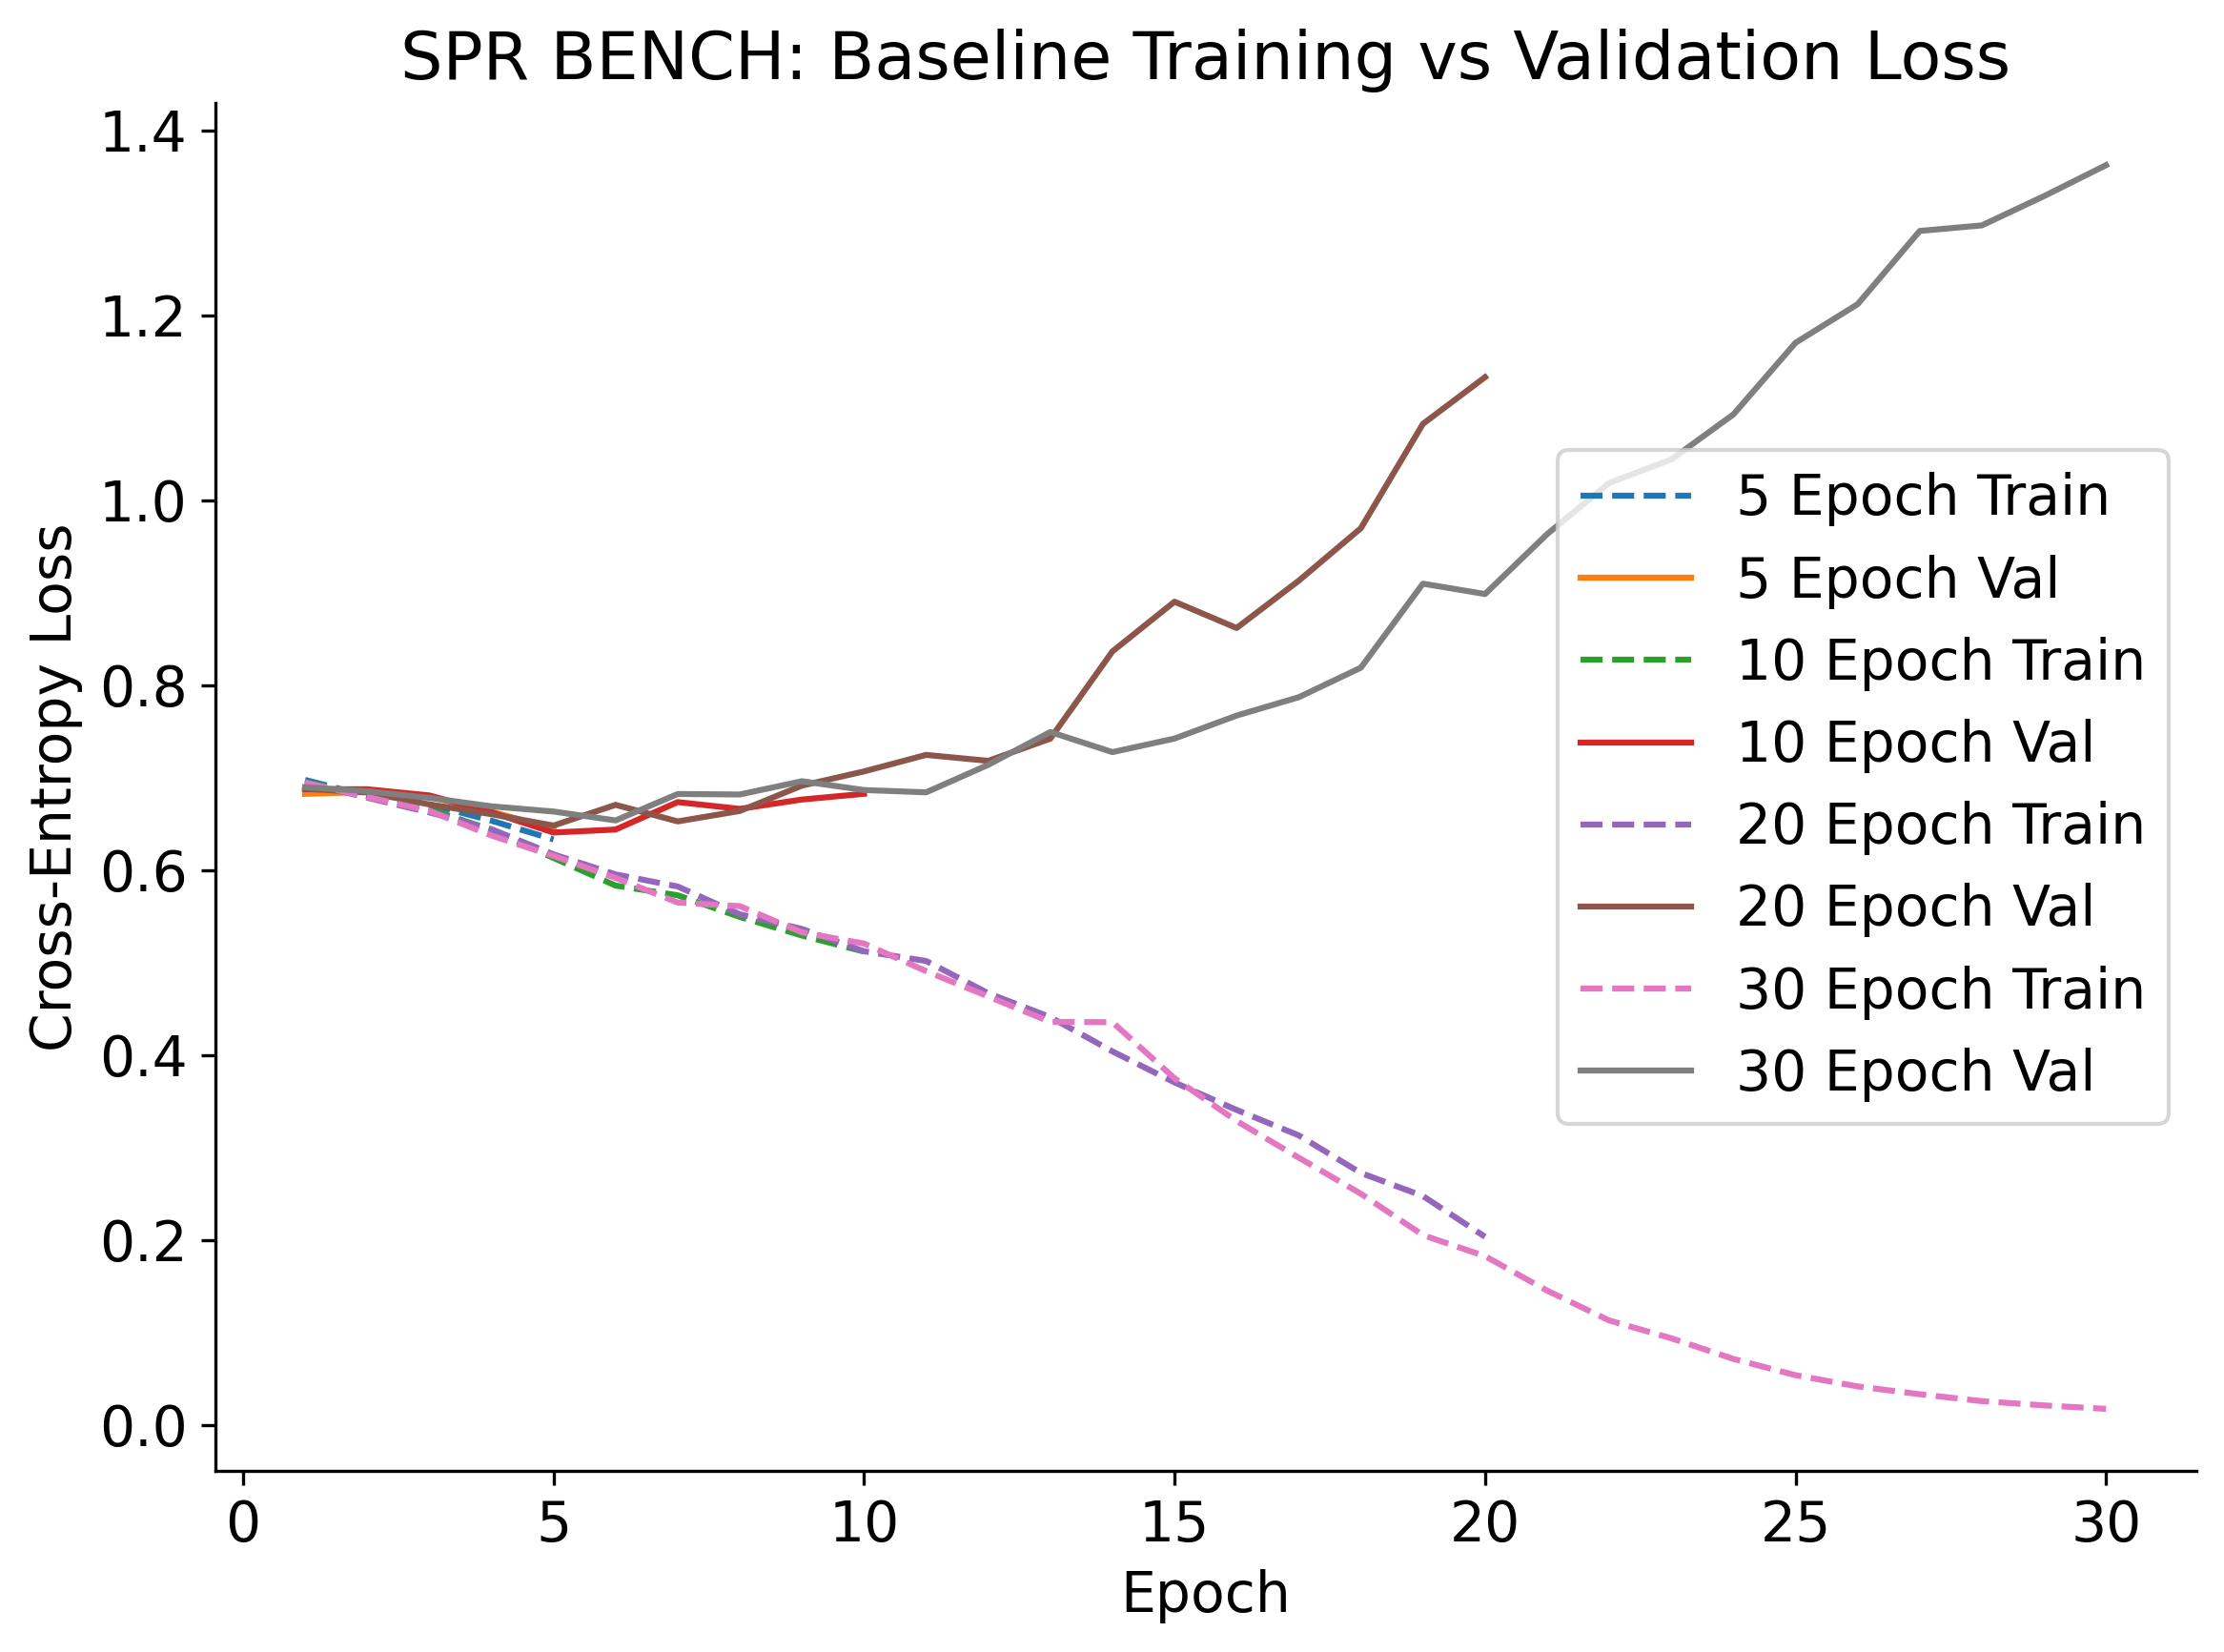
\includegraphics[width=\textwidth]{Baseline_Loss_Curves.png}
  \caption{Loss curves over training epochs.}
\end{subfigure}
\hfill
\begin{subfigure}[b]{0.45\textwidth}
  \centering
  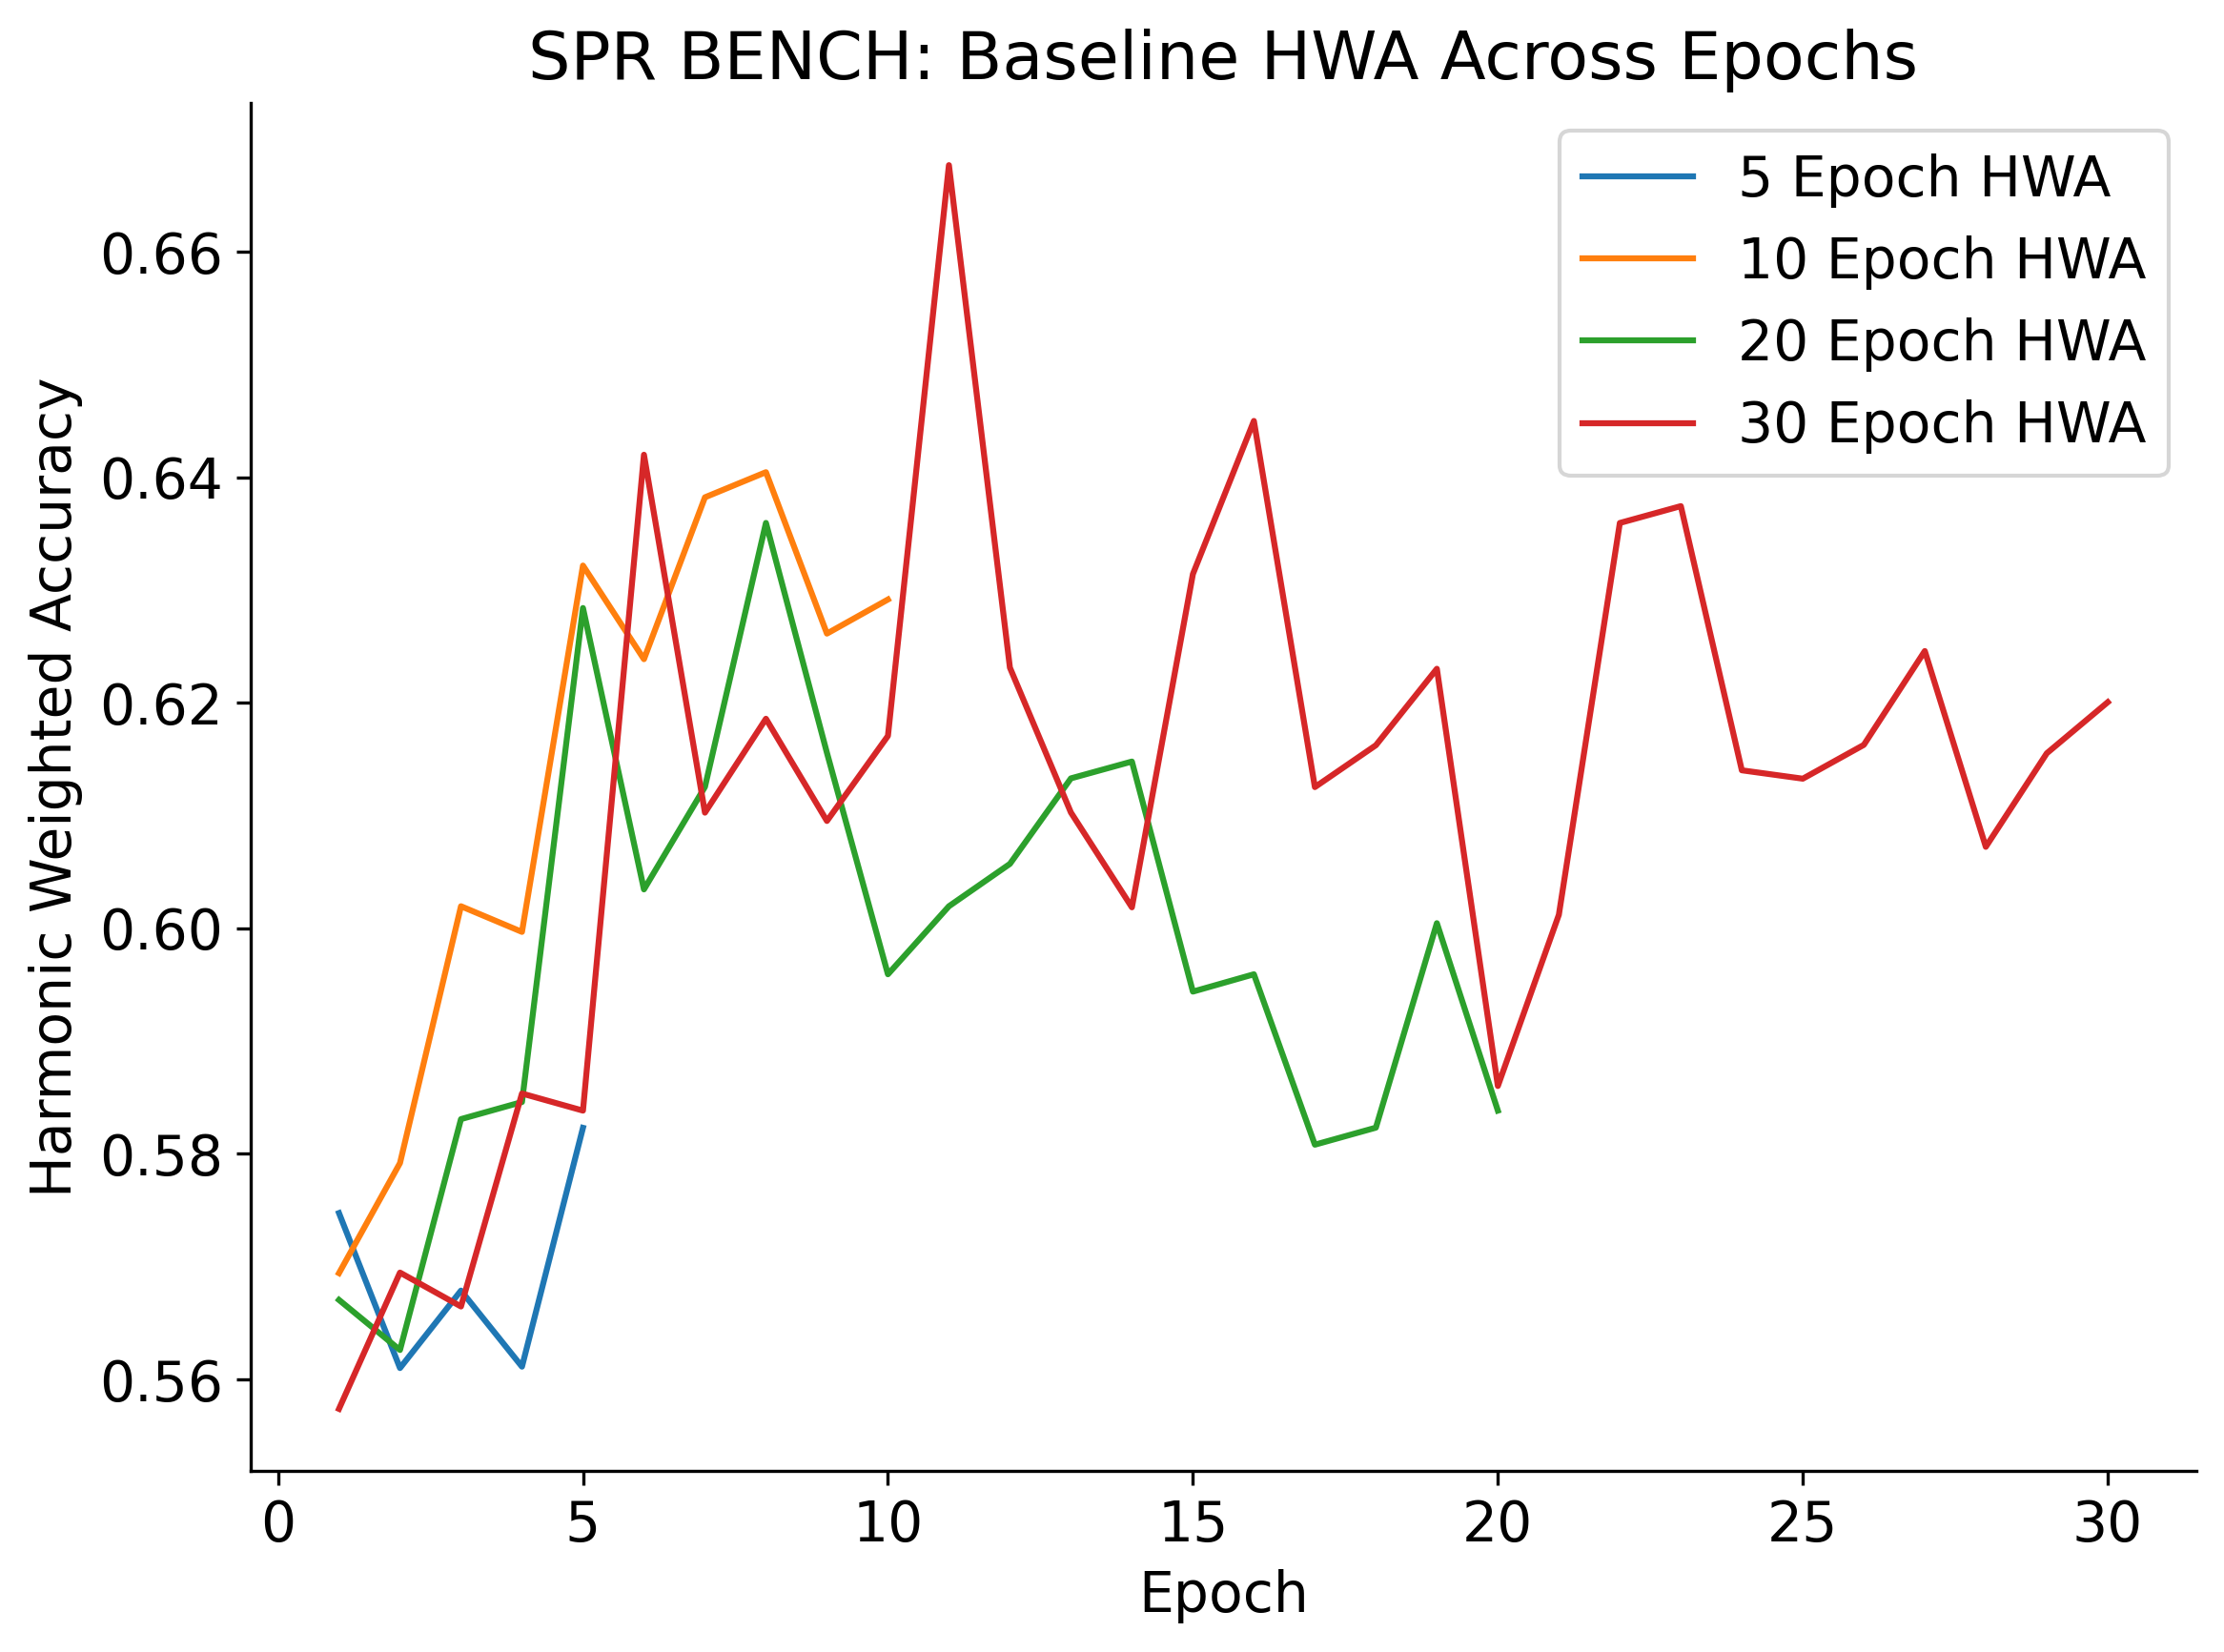
\includegraphics[width=\textwidth]{Baseline_HWA_Curves.png}
  \caption{Held-out accuracy plateaus early.}
\end{subfigure}
\caption{Our baseline model quickly overfits, with gains in train loss not reflected in the held-out metric.\label{fig:baseline_curves}}
\vspace{-1em}
\end{figure}

We confirmed that slight modifications to the tokenization or embedding freeze strategy led to abrupt changes in learning. These observations emphasize the ease with which performance can appear improved in lab settings when key hyperparameters are omitted or incorrectly reported.

\section{Conclusion}
We presented insights gathered from a sequence analysis task in which minor data or architecture changes led to unreliable generalization. Our negative and inconclusive results caution that single-run improvements or unseen confounding factors can mask deeper weaknesses in model design. Future work could systematically examine how multi-seed variability correlates with real-world readiness.

\bibliographystyle{plainnat}
\bibliography{references}

\appendix
\section{Appendix}
Here, we expand on technical details and provide additional figures relevant to architecture and ablation comparisons. Figure~\ref{fig:lstm} visualizes a bidirectional LSTM we tested, and Figures~\ref{fig:context_abl}a-c illustrate context ablation setups (e.g., randomizing token order, isolating shape vs.\ color). While informative, these analyses revealed no systematic performance improvements relative to our baselines, underscoring that many variations produced partially negative or inconclusive results.

\begin{figure}[h]
    \centering
    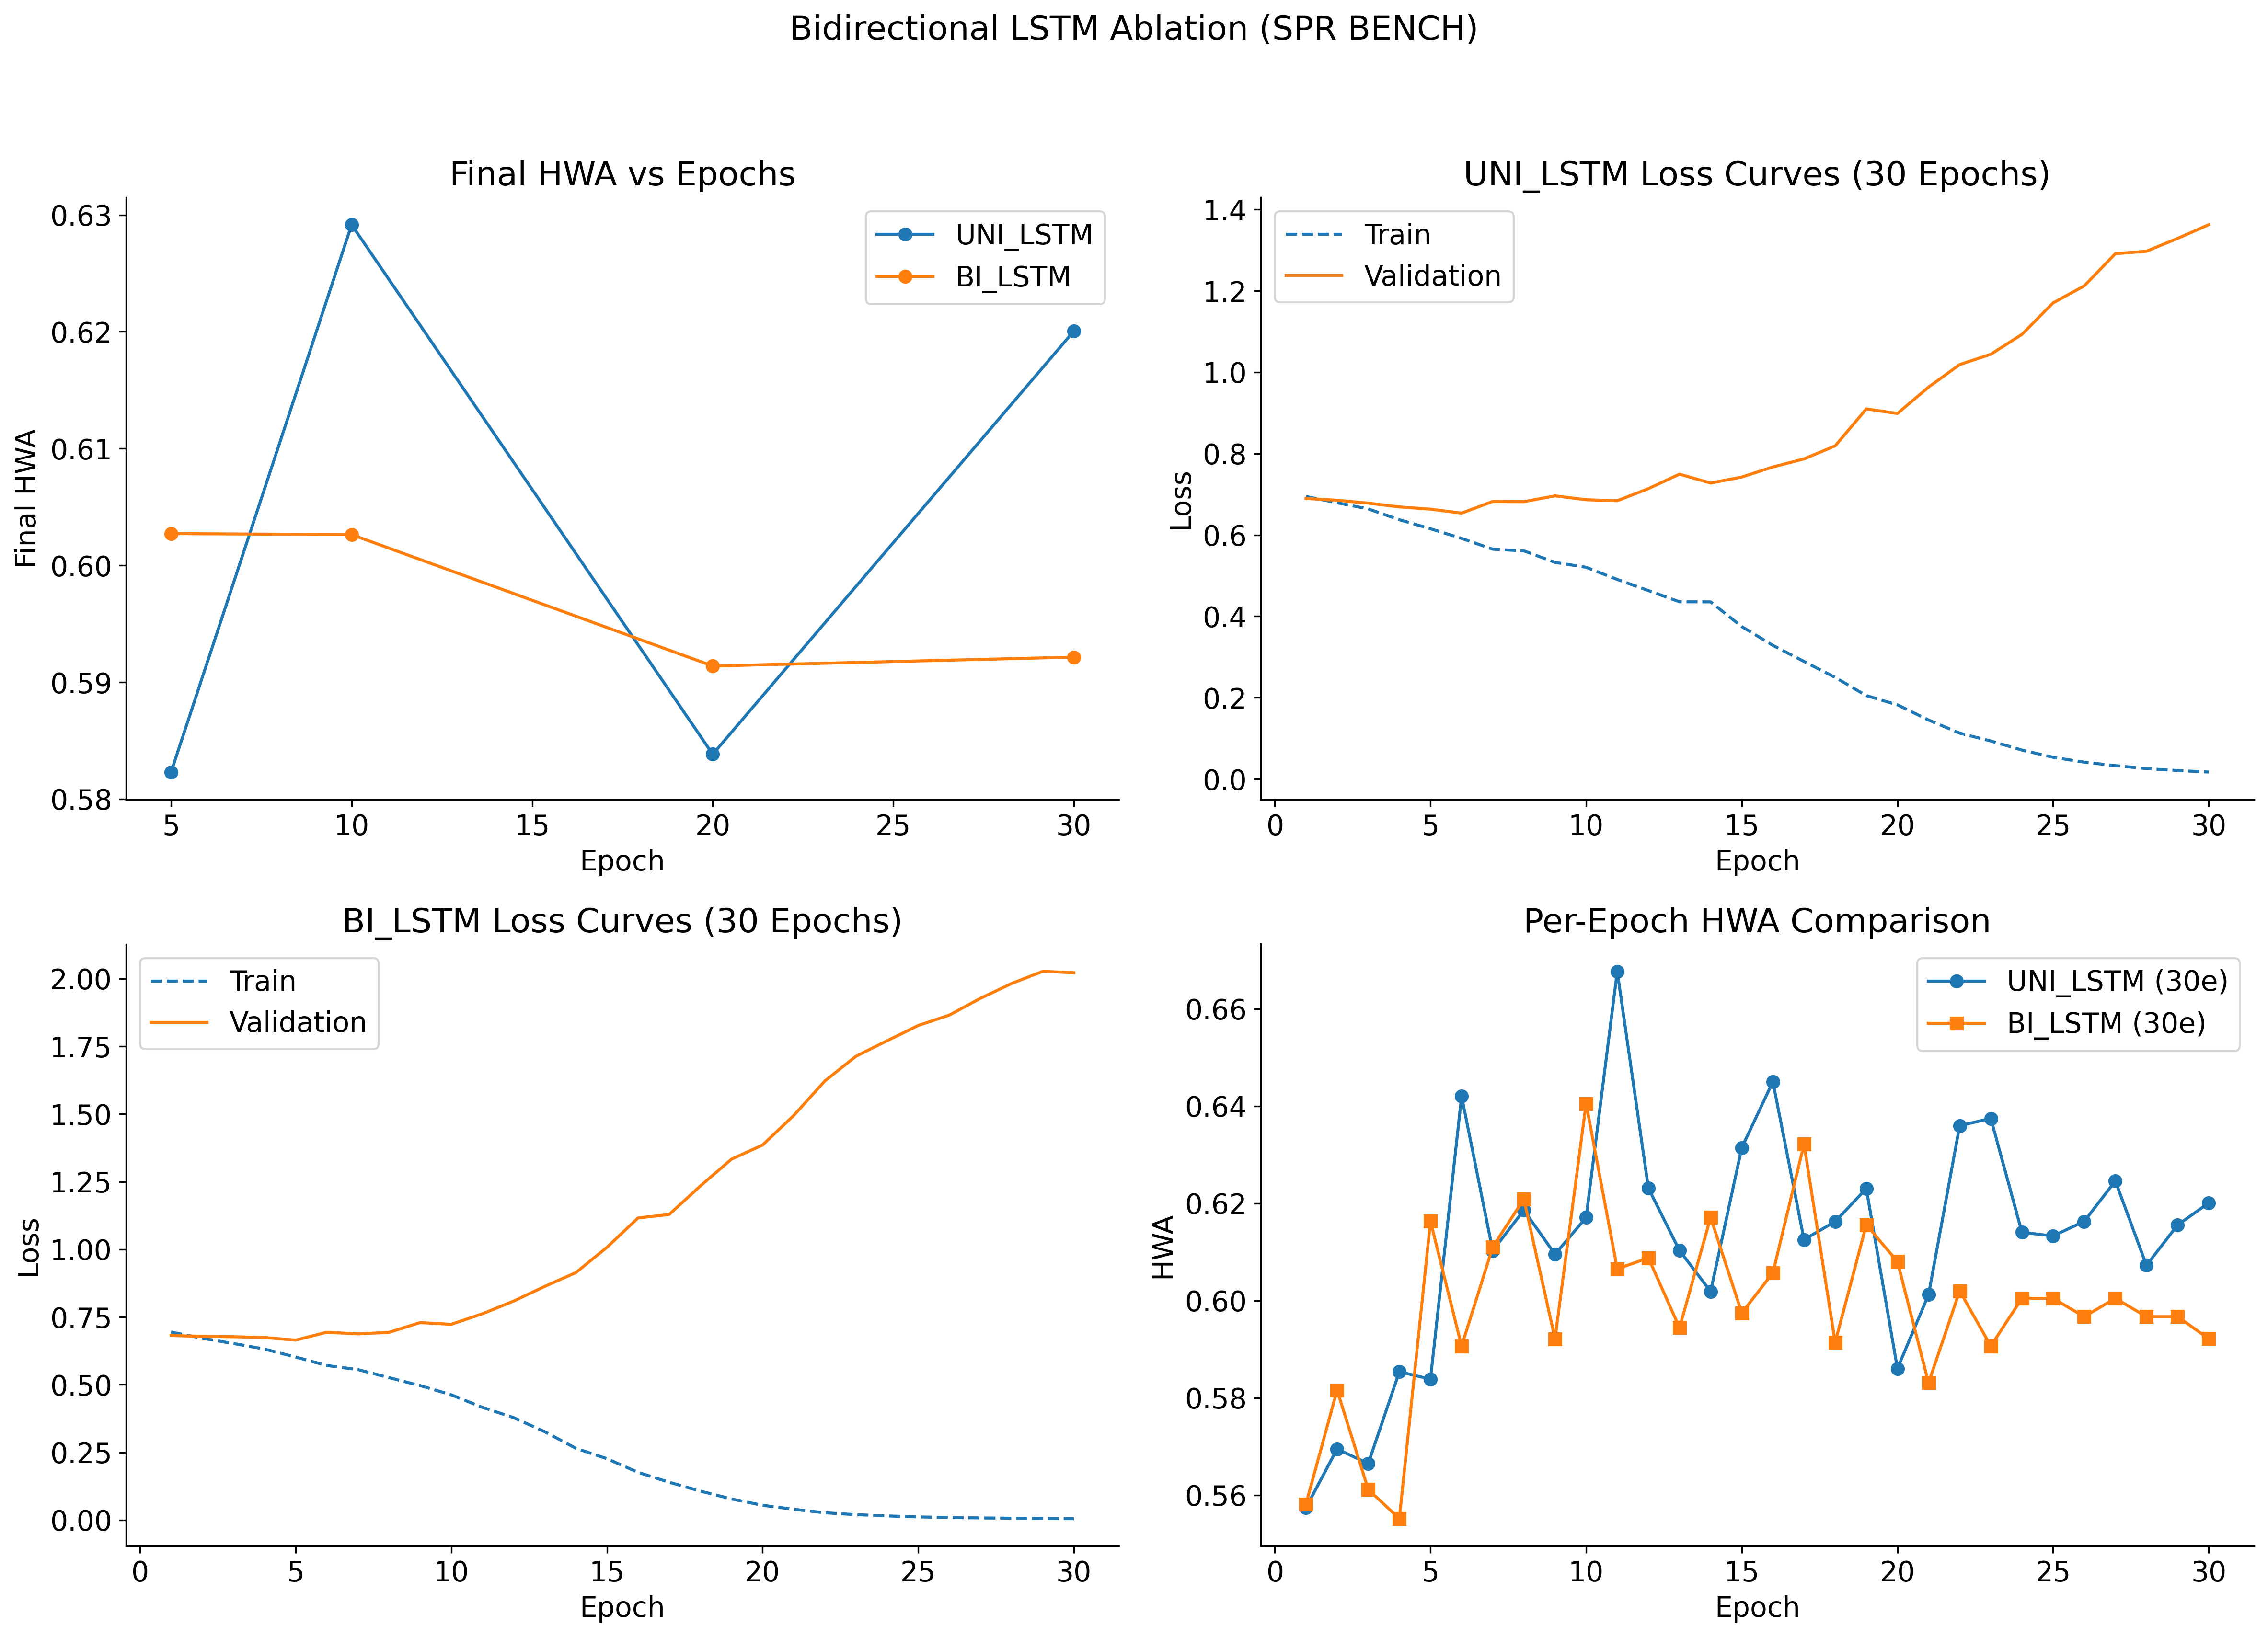
\includegraphics[width=0.3\textwidth]{Bidirectional_LSTM.png}
    \caption{A bidirectional LSTM used in additional experiments.\label{fig:lstm}}
\end{figure}

\begin{figure}[h]
    \centering
    \minipage{0.32\textwidth}
      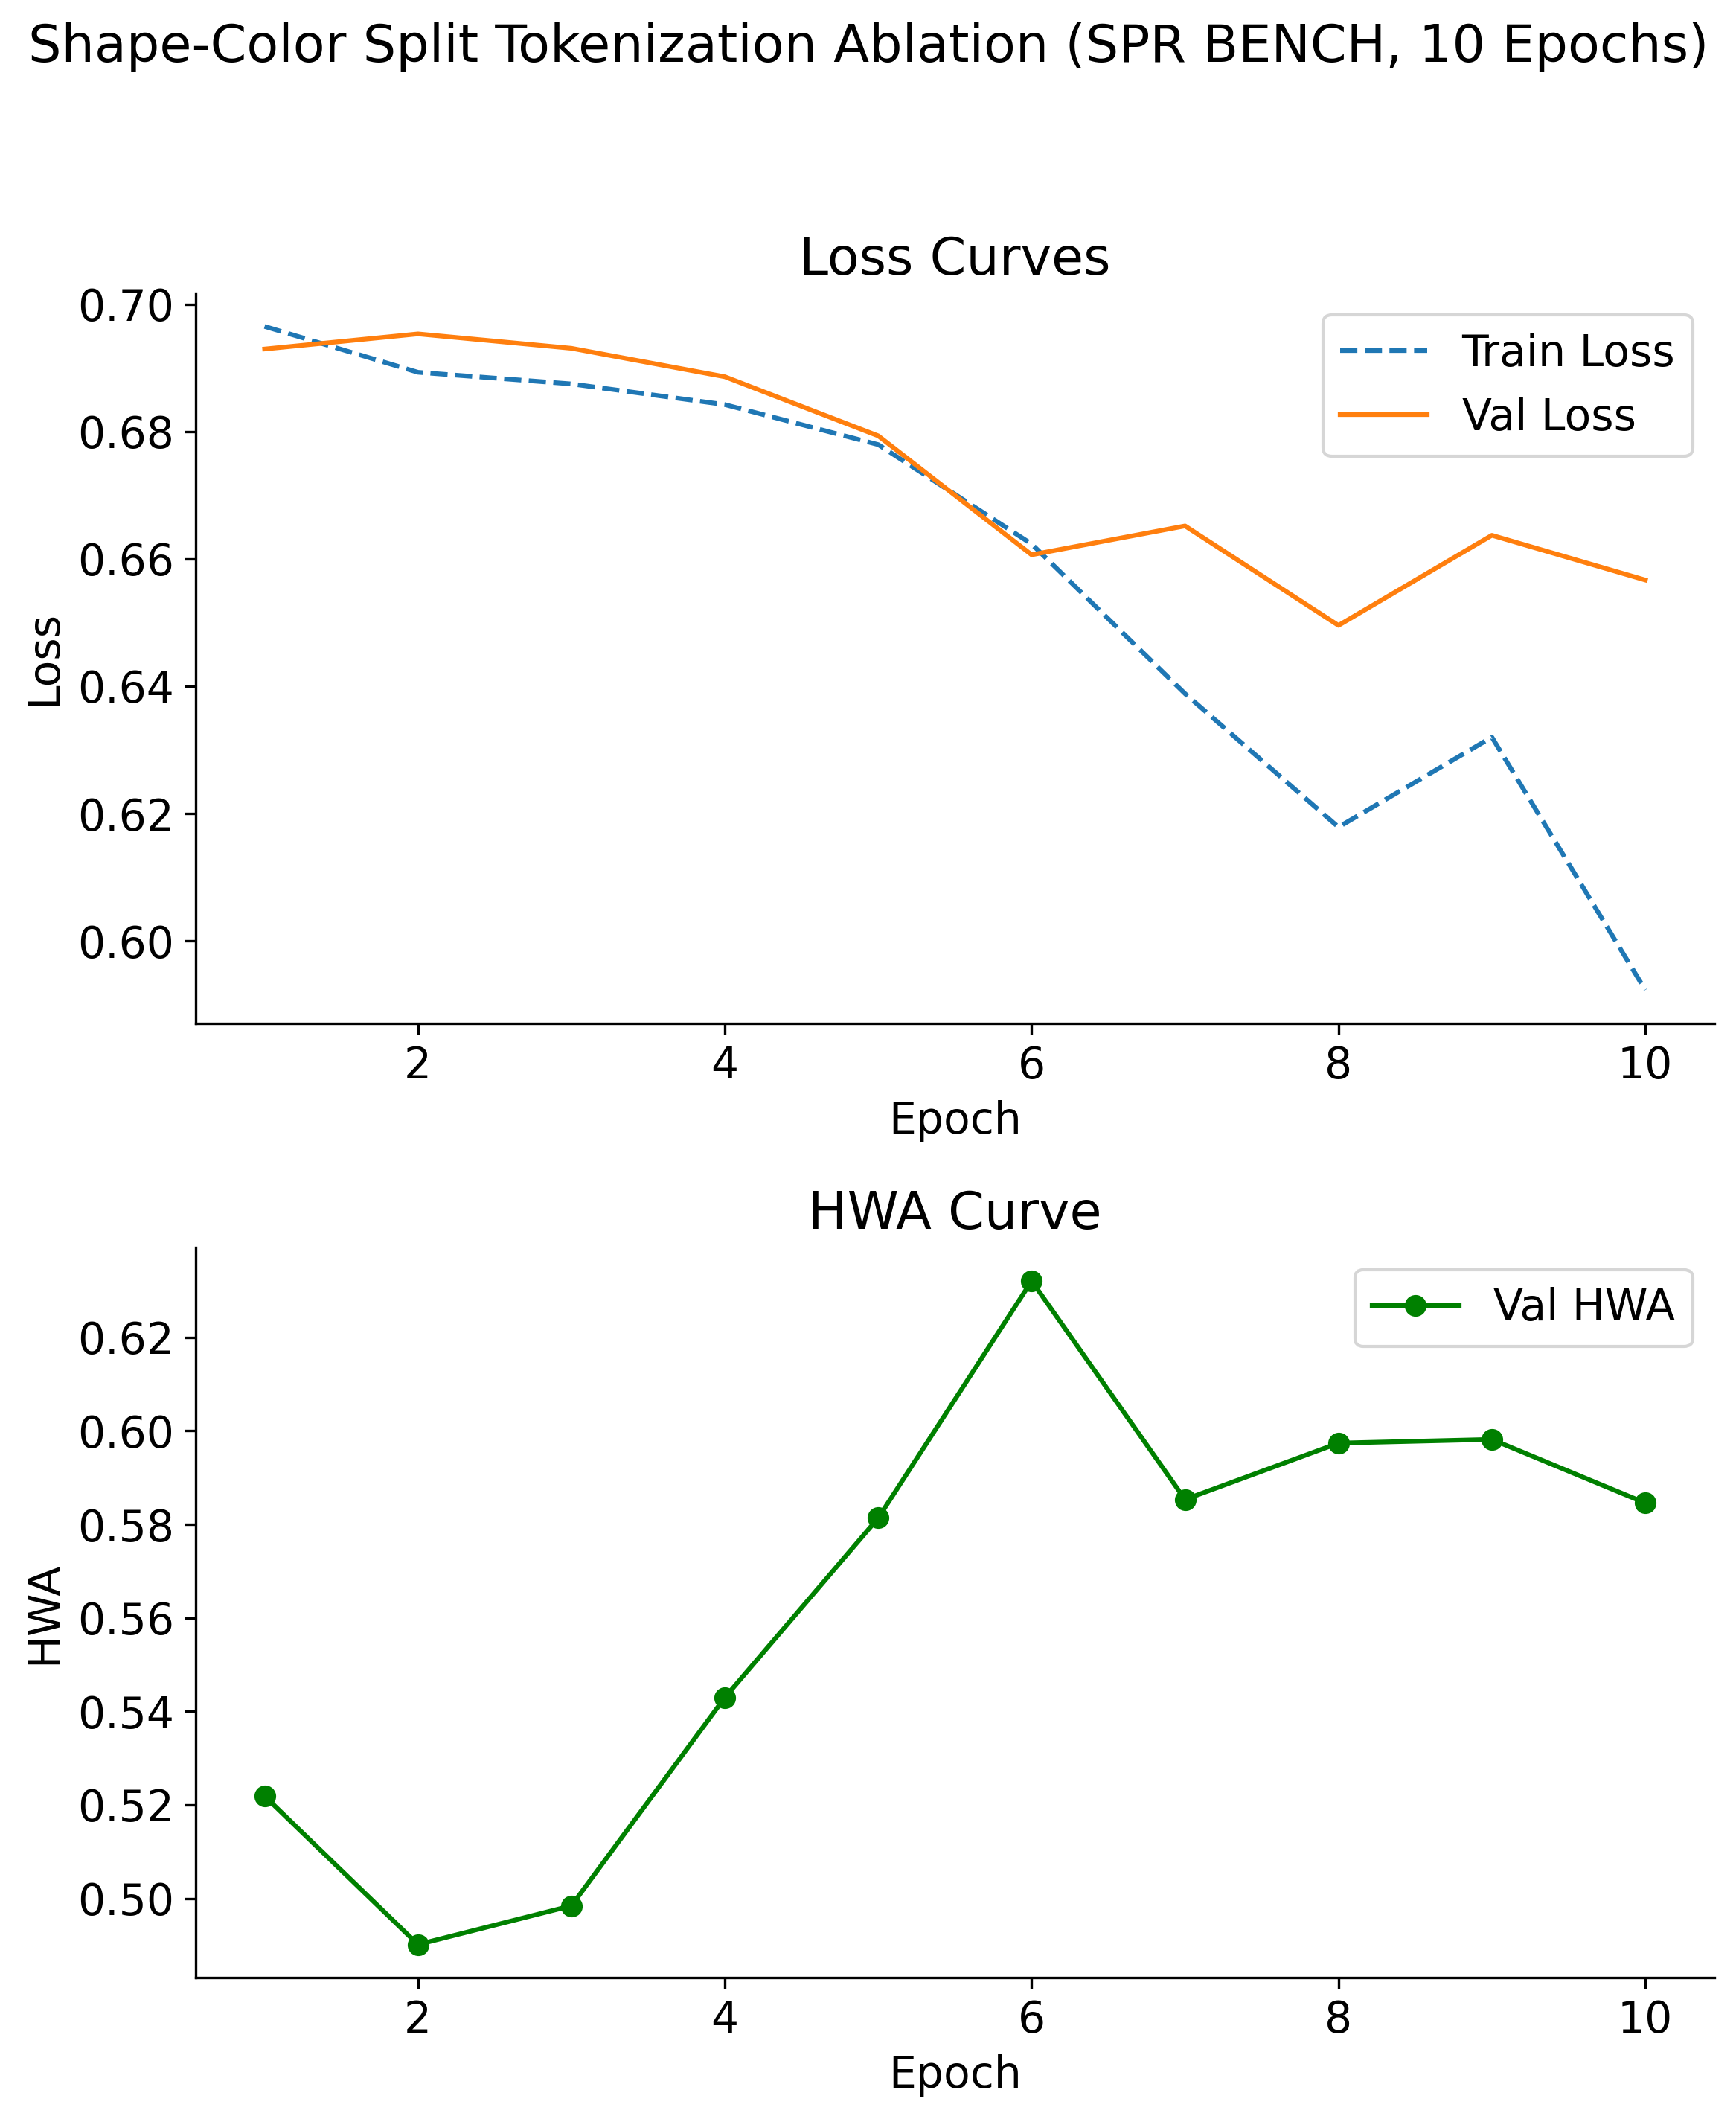
\includegraphics[width=\linewidth]{ShapeColor_Split.png}
    \endminipage
    \minipage{0.32\textwidth}
      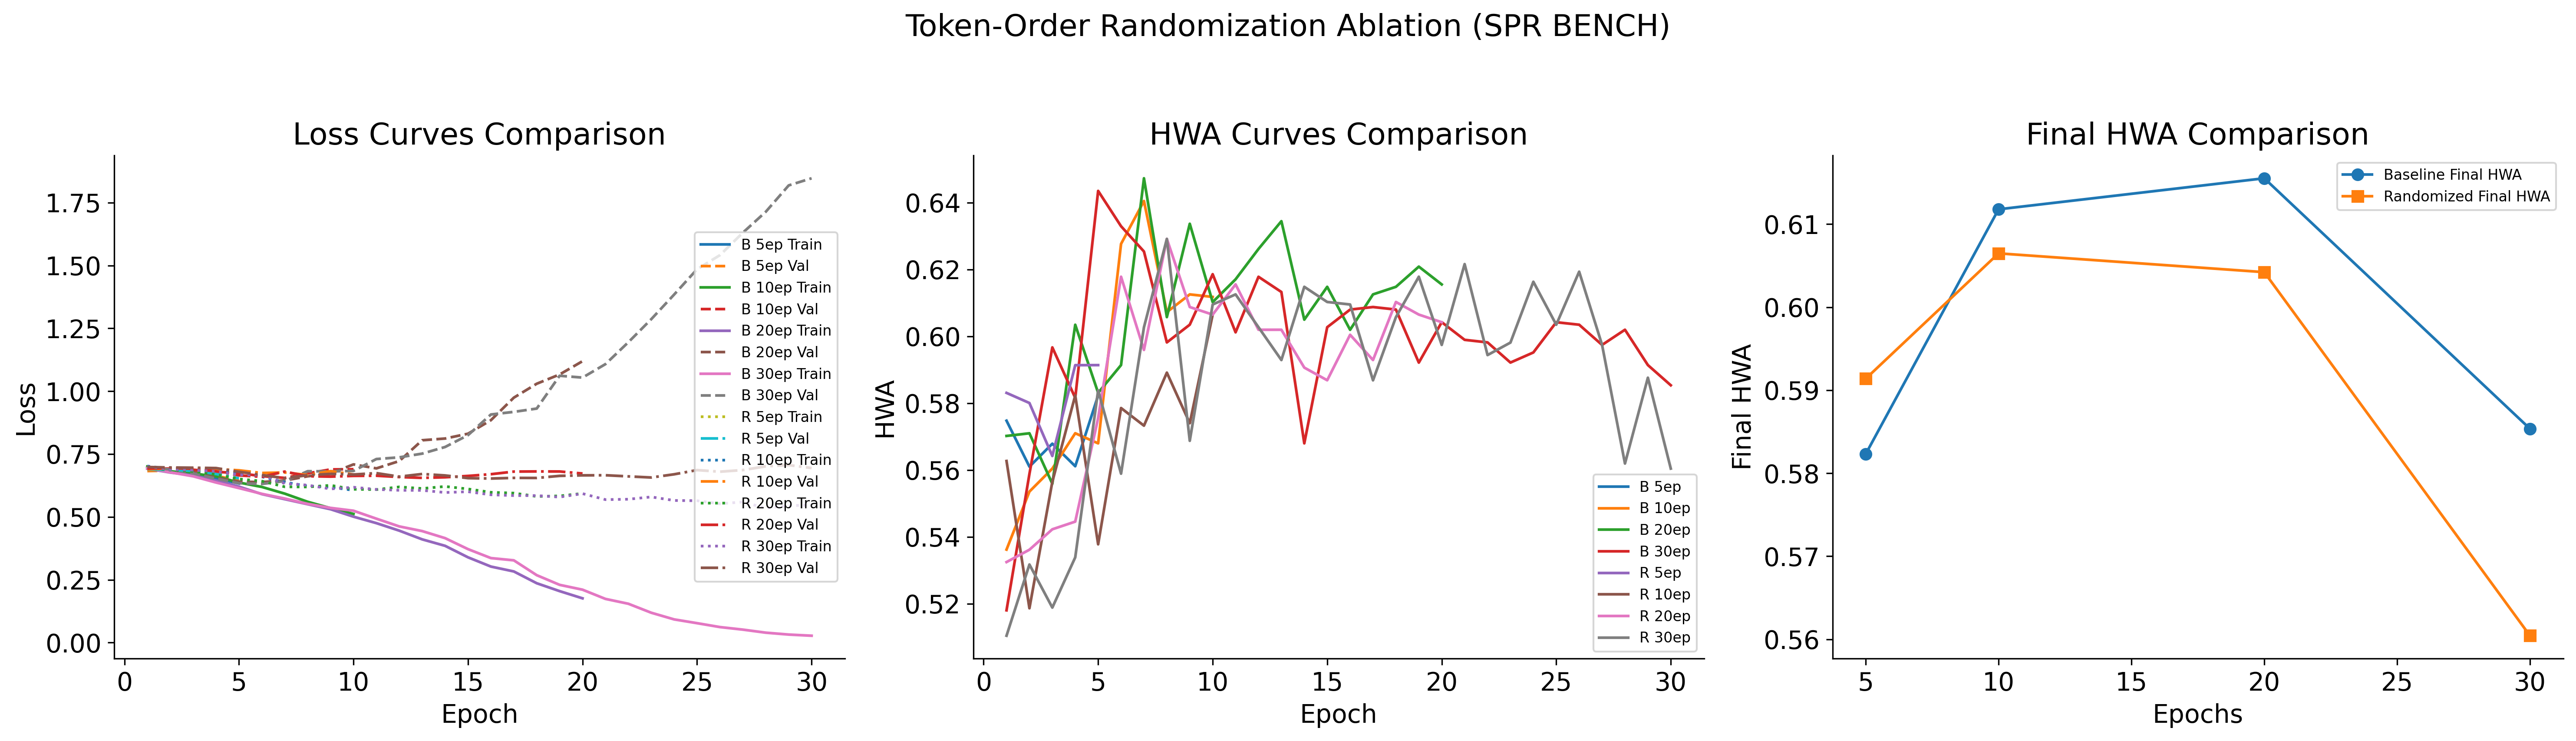
\includegraphics[width=\linewidth]{TokenOrder_Randomization.png}
    \endminipage
    \minipage{0.32\textwidth}
      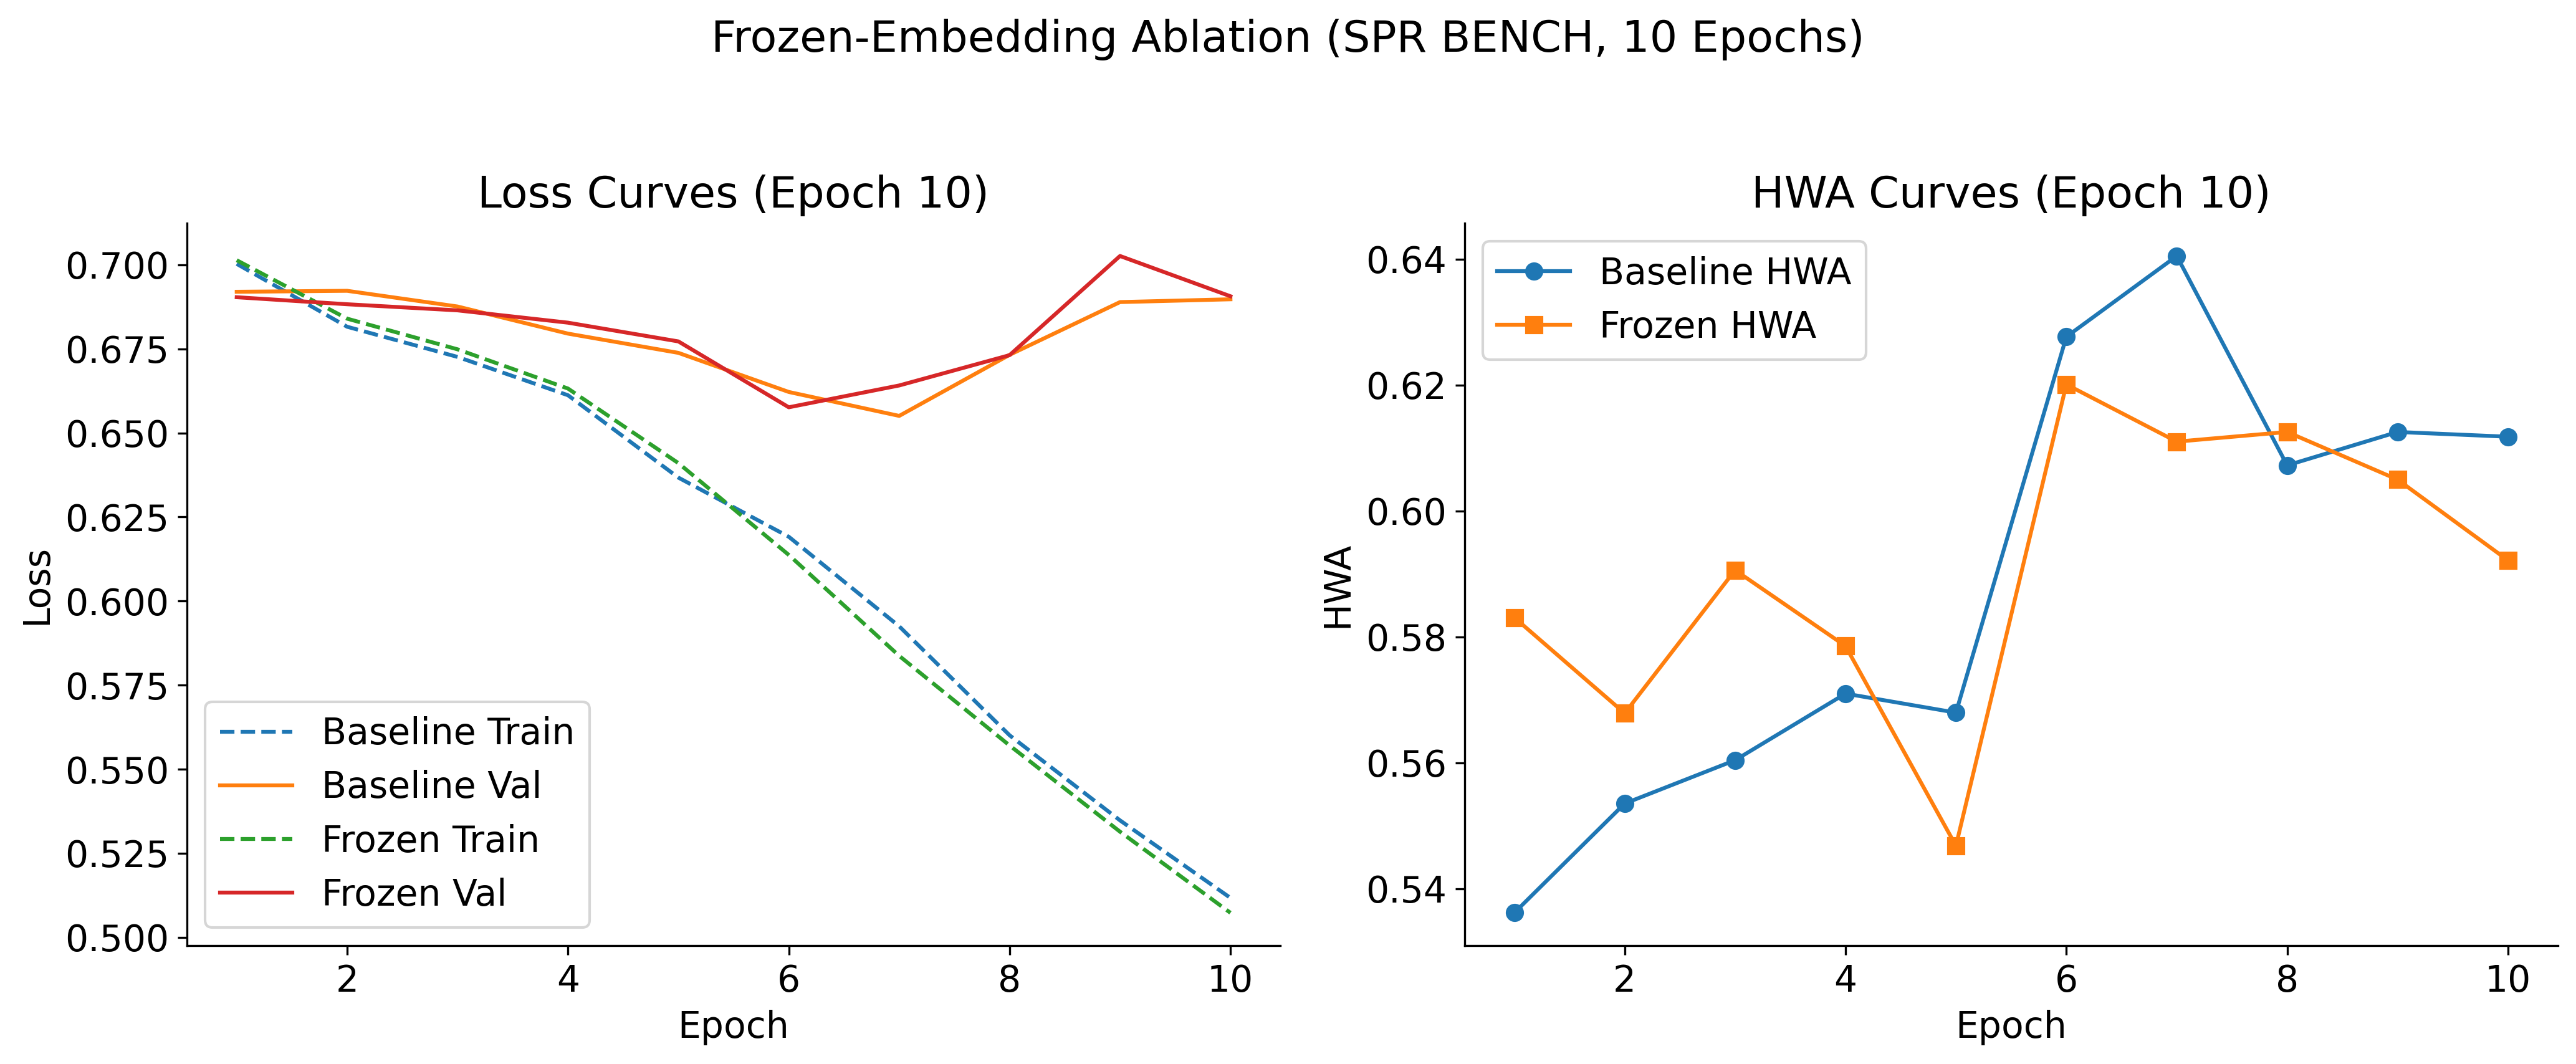
\includegraphics[width=\linewidth]{FrozenEmbedding_Ablation.png}
    \endminipage
    \caption{Context ablation illustrations.\label{fig:context_abl}}
\end{figure}

\clearpage

\begin{filecontents}{references.bib}
@misc{t5,
  title={Exploring the Limits of Transfer Learning with a Unified Text-to-Text Transformer},
  author={Raffel, Colin and Shazeer, Noam and Roberts, Adam and Lee, Katherine and Narang, Sharan and Matena, Michael and Zhou, Yanqi and Li, Wei and Liu, Peter J.},
  year=2020,
  howpublished={arXiv:1910.10683 [cs.LG]}
}
\end{filecontents}

\end{document}